\section{Simultaneous connect}
\begin{frame}{Simultaneous connect}
  \begin{itemize}
    \item Multiple startup
    \item Multiple connect
  \end{itemize}
\end{frame}

\begin{frame}{Simultaneous connect}
\framesubtitle{Model Performance}
  \begin{figure}[ht]
  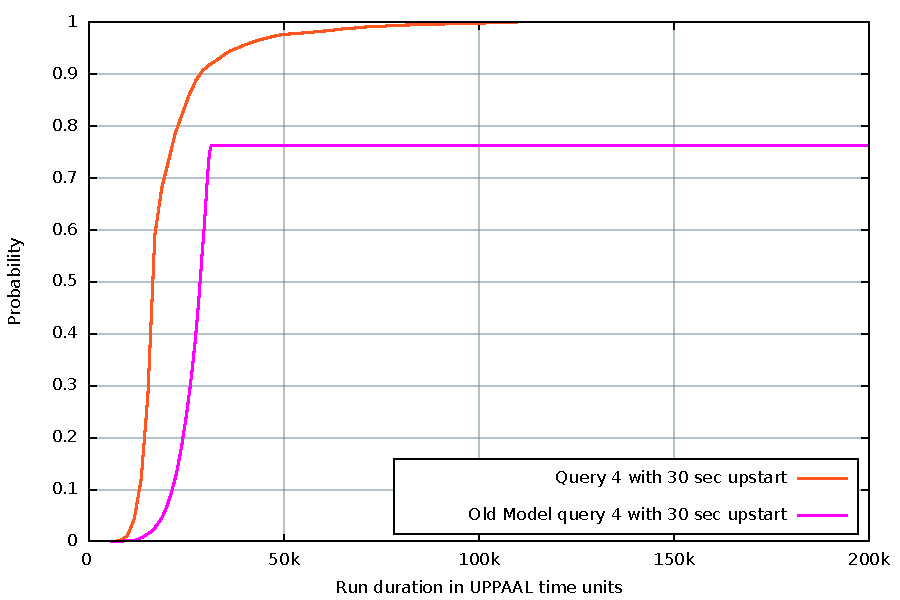
\includegraphics[width=1\textwidth]{images/graph.pdf} 
\caption{Graph of the UPPAAL SMC queries, in which the cumulative probability increase over time. With 99.9 \% confidence and five devices.}
\label{fig:ConnectQueryTime}
\end{figure}
\end{frame}

\section{CCUC}
\subsection{CCUC assumptions}
\begin{frame}{CCUC assumptions}
The CCUC-problem describes a completely connected graph but in this scenario there is not a guarantee that the transmission will be received; all devices are still in the range of each other.
\end{frame}

\subsection{CCUC Solution}
\begin{frame}{CCUC Improvements}
\framesubtitle{Message Redundancy}
\only<1>{
  \begin{itemize}
    \item Pros
      \begin{itemize}
    	\item Increases reliability
    	\item Simple to implement
  	  \end{itemize}
    \item Cons
      \begin{itemize}
    	\item Time consuming
    	\item Naïve solution
  	  \end{itemize}
  \end{itemize}
}
\only<2>{
\begin{figure}%{\linewidth}
\centering
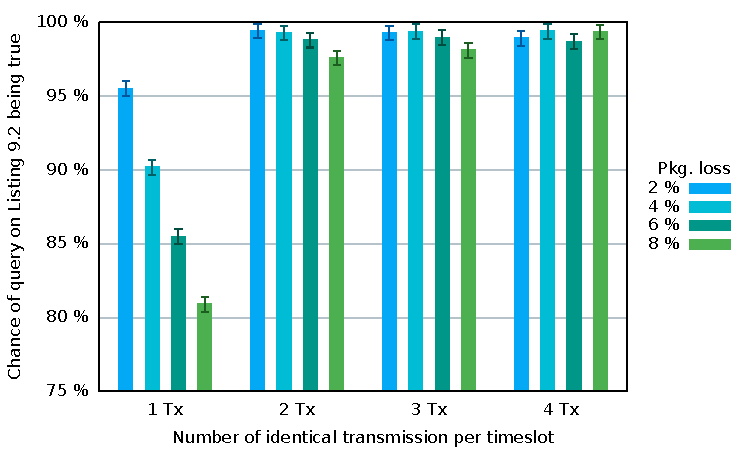
\includegraphics[width=1\textwidth]{images/graph2.pdf} 
\caption{Miss chances with CCUC solution}
\label{CCUC-Graph-UPPAAL}
\end{figure}

}
\only<3>{
\begin{figure}
\centering
\begin{tikzpicture}  [
        node distance = 1 cm, 
        vertex/.style = {circle, draw, fill=blue!10}, 
        label/.style = {fill=white},
        block/.style = {rectangle, draw, fill=orange!40, minimum height = 5mm, minimum width = 20mm}
    ]

    \node[draw=none](0){};
    \node[vertex, above =     of 0]   (2) {$v_1$};
    \node[block,  below = 9mm of 2]   (1) {};
    \node[vertex, right = 2cm of 0]   (3) {$v_2$};
    \node[vertex, below =     of 0]   (4) {$v_3$};
    
    \draw [<->] (2) -- (3);
    \draw [<->] (3) -- (4);
    \draw [->] 	(1) -- (2);
    \draw [->] 	(1) -- (4);
    \draw [opacity=0.5] (1.south) -- (1.north);

\end{tikzpicture}
\end{figure}
Likely real world scenario
}
\end{frame}
